\documentclass[10pt, aspectratio=43]{beamer}
\usepackage[utf8]{inputenc}
\usepackage{wasysym}
\usepackage{booktabs}
\usepackage{tabu}

\renewcommand{\arraystretch}{1.2}

\mode<presentation> {
\usetheme{Massey}
\usecolortheme{DarkLetters}

% Now load other modules
\usefonttheme{professionalfonts}
% To get running page numbers in all slides uncomment this line
% To get a header in all slides uncomment this line
%\headlinecontent{Text left top corner}{Text top center}
}
\setbeamertemplate{footline}[frame number]
\setbeamercolor{subsubsection in toc}{fg=black}
\setbeamertemplate{section in toc shaded}[default][90]

%----------------------------------------------------------------------------------------
%	TITLE PAGE
%----------------------------------------------------------------------------------------

\title{Statistical Analysis Pipeline} 
\suptitle{Admixture Data from a Human Population Settlement Model}
\author{Aurélien \textsc{Luciani}}
\department{Master 2 Bioinformatique}
\institute{Université de Bordeaux}
\date{11 September 2015}

%=================================================  START DOCUMENT ======================================

\begin{document}

% Default values for the Massey branding will be used
% \masseyBrand[fillcolour]{framedesign}[opacity]{picture}{masseylogo}{enginelogo}[frametitlecolour]
\masseyBrand{}{../data/background-2.png}{}{}

% Massey styled title -------------------------------------------------------------------------

%\masseyBrand{bar}{picturefilename}{blueletters}{blueletters}{}

\begin{frame}[t, noframenumbering]  % The [t] is important!!!!
\masseyTitlepage

\raggedleft
\begin{mblock}[140pt]{0.7}{}
\raggedleft
\textbf{\insertauthor}\\
\insertdepartment\\
\insertinstitute\\
\insertdate
\end{mblock}
\vfill
\begin{mblock}[300pt]{0.7}{}

\includegraphics[width=0.5\textwidth]{uniLogo/MasseyLogoBlueLetters.png}%

\includegraphics[width=0.5\textwidth]{../data/ub.jpg}
\end{mblock}
\end{frame}

% Slides ---------------------------------------------------------------------------------

\section*{Introduction}
\masseyBrand{}[1]{../data/nz.png}{}{}
\begin{frame}{}{Introduction}
\vspace*{0.5cm}
\begin{columns}
  \column{0.2\textwidth}
  
  \column{0.8\textwidth}
  \color{white}
  \begin{itemize}
    \item Internship at Massey University (New Zealand)
    \item Computational Biology Research Group
    \item Part of a 2 years project
    \item Research assistant for the project:
    \begin{itemize}
      \item François Vallée
    \end{itemize}
    \item Supervisors:
    \begin{itemize}
      \item Murray Cox
      \item Marie Noelle Beurton-Aimar
    \end{itemize}
  \end{itemize}

\end{columns}
\end{frame}

% Change background if needed
%\masseyBrand[fillcolour]{full/bar}[opacity]{picture}{blueletters/whiteletters}{blueletters/whiteletters}[frametitlecolour]
\section{Context}
\masseyBrand{bar}[0.1]{}{}{}
\begin{frame}{}{Table of contents}
\tableofcontents[currentsection, sectionstyle=show/shaded, subsectionstyle=show/show/hide]
\end{frame}

\subsection{Geological and anthropological context}
\masseyBrand{}{../data/background-2.png}{}{}
\begin{frame}{}{}
\end{frame}

\addtocounter{framenumber}{-1}
\masseyBrand{}{../data/background-3-first-wave.png}{}{}
\begin{frame}{}{First settlement wave Around 45,000 years ago}
\vspace*{-0.8cm}
\begin{columns}
  \column{0.65\textwidth}

  \column{0.52\textwidth}
  \color{masseyWhite}
  \begin{itemize}
    \item First humans
    \item Ancestral Melanesian population
    \item Hunter-gatherers
  \end{itemize}

\end{columns}
\end{frame}

\addtocounter{framenumber}{-1}
\masseyBrand{}{../data/background-2-second-wave.png}{}{}
\begin{frame}{}{Second settlement wave Around 4,500 years ago}
\vspace*{-0.8cm}
\begin{columns}
  \column{0.65\textwidth}

  \column{0.52\textwidth}
  \color{masseyWhite}
  \begin{itemize}
    \item “Austronesian expansion”
    \item Two possible waves
    \item Admixture between populations
    \item What started it?
    \begin{itemize}
      \item Agriculture knowledge?
      \item Better navigation?
    \end{itemize}
  \end{itemize}

\end{columns}
\end{frame}

\subsection{Previous papers}
\masseyBrand{bar}[0.1]{}{}{}
\begin{frame}{Context}{Previous papers}
\begin{columns}
  \column{0.6\textwidth}
  \begin{figure}
    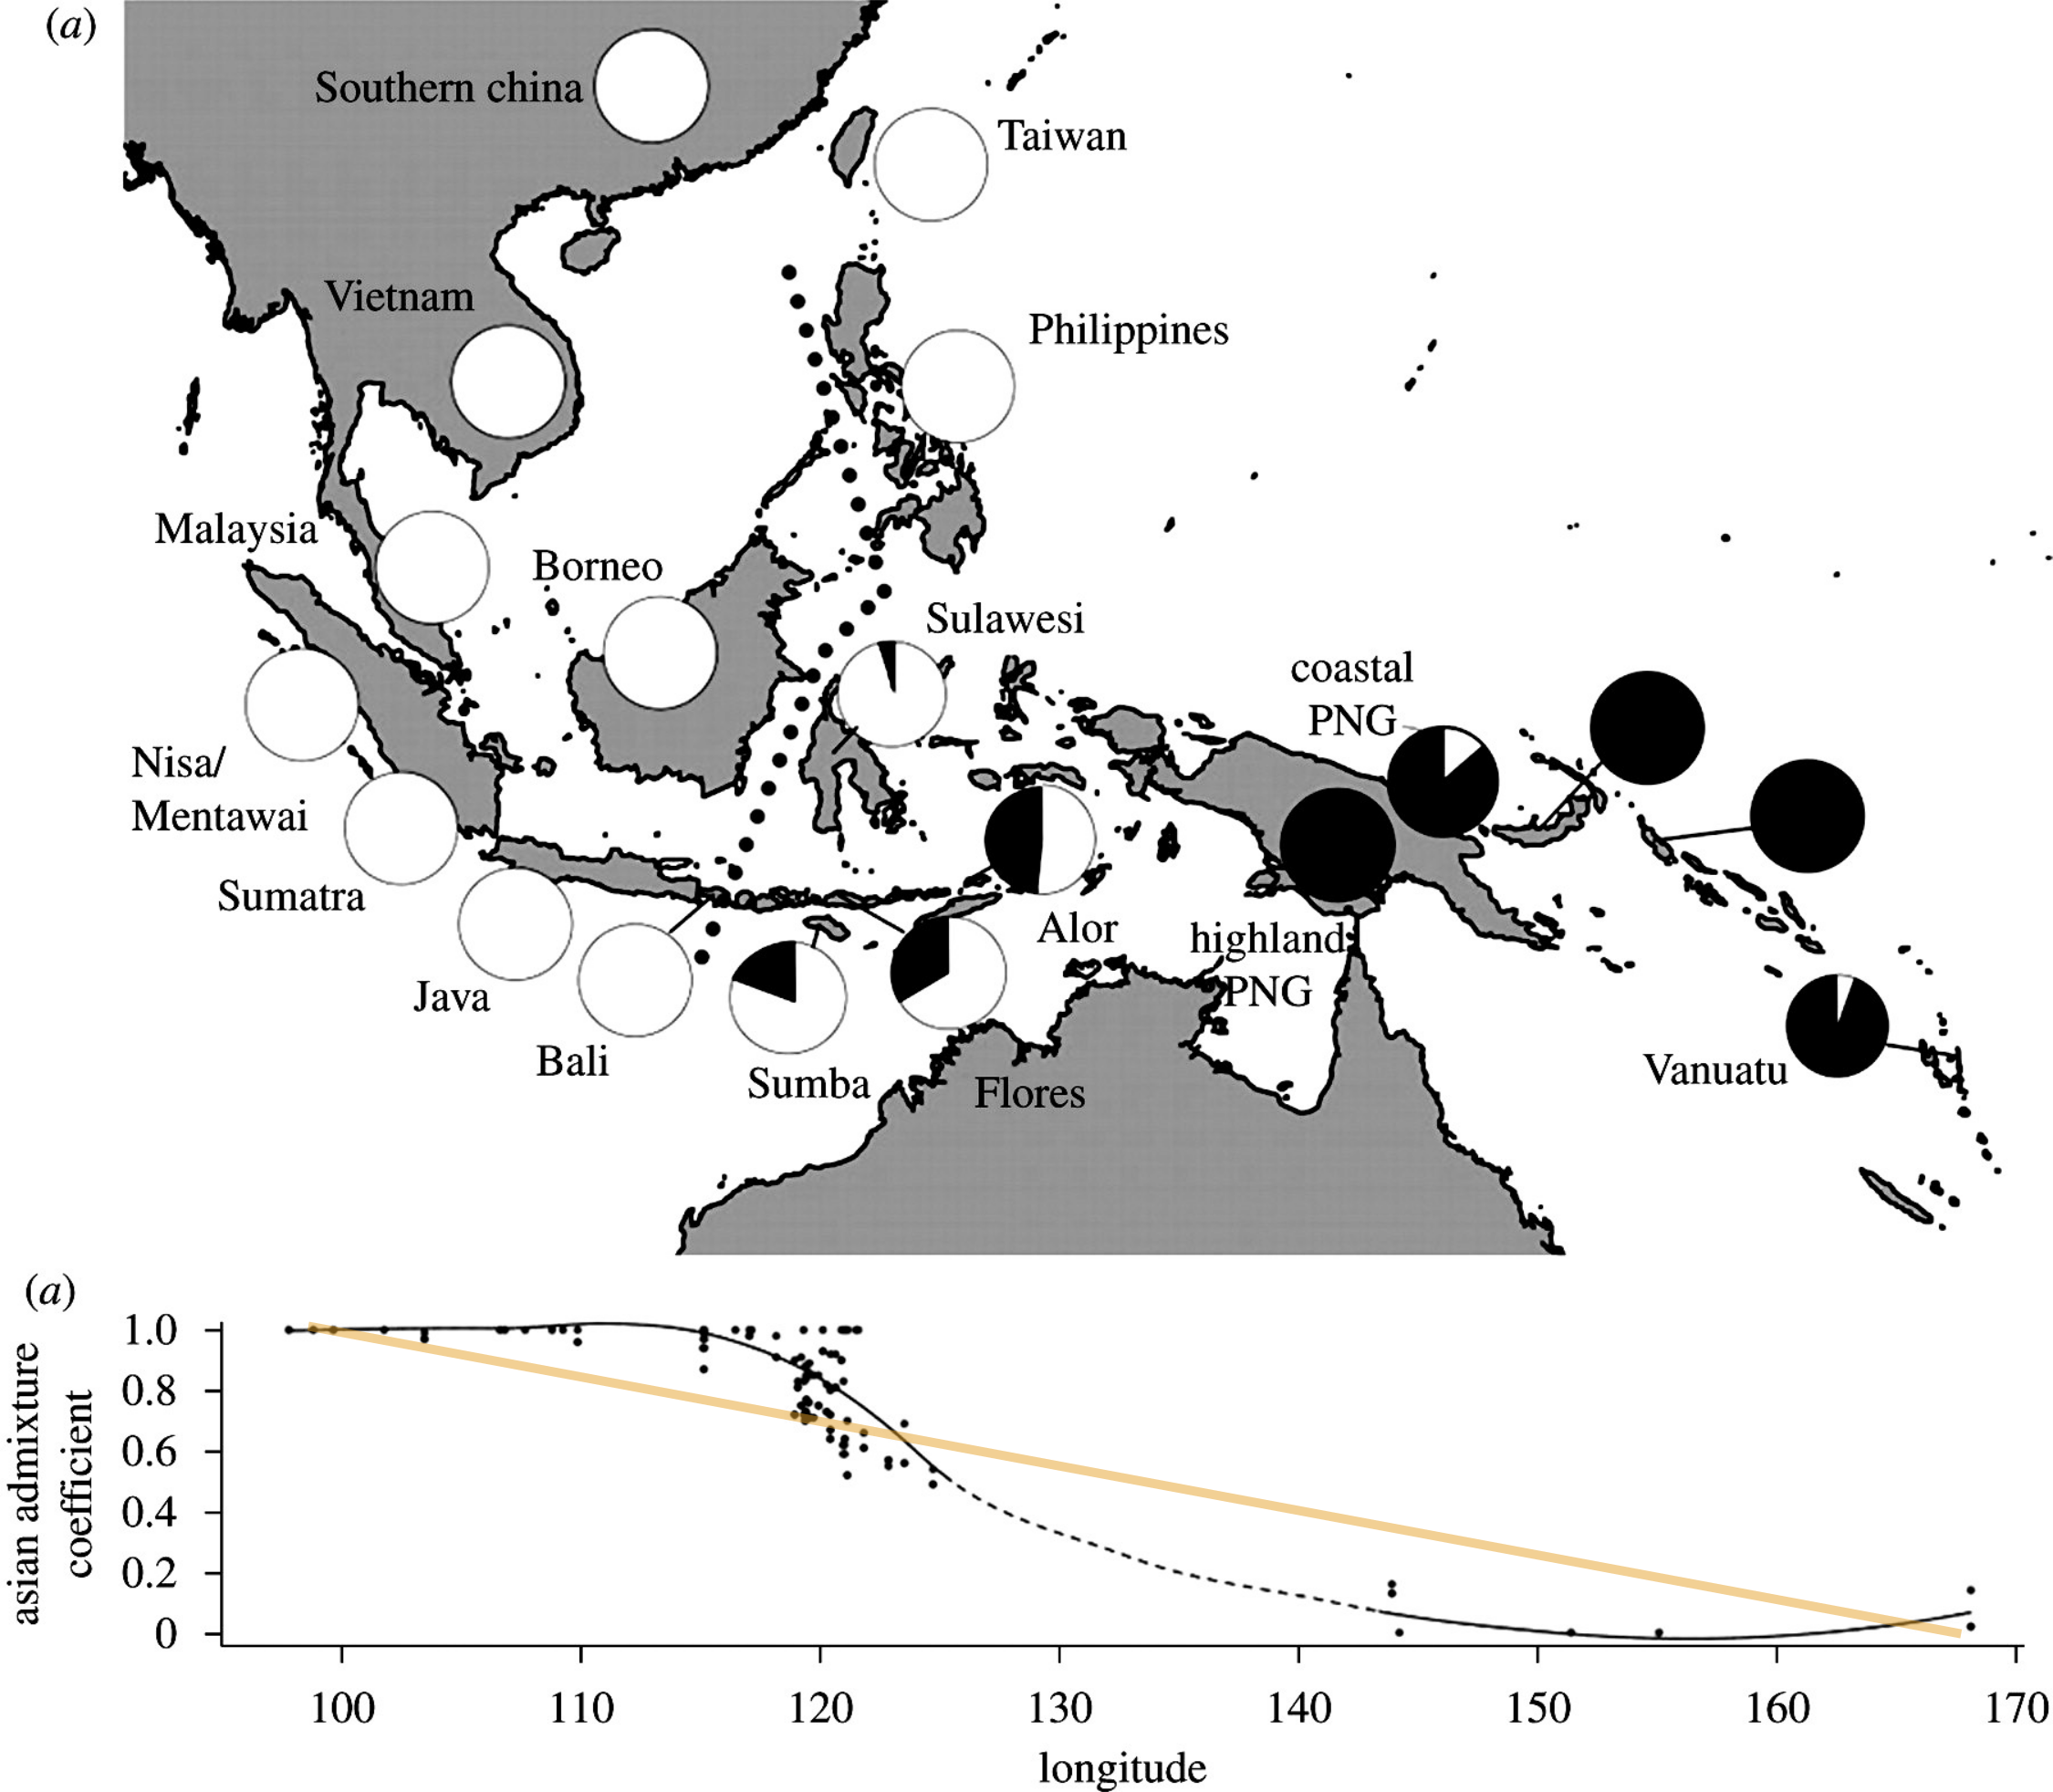
\includegraphics[width=0.95\textwidth]{../data/cox-image-modified.jpg}
    \caption{Cox et al. [2010]. \textit{Proceedings of
the Royal Society of London B: Biological Sciences}, modified}
  \end{figure}

  \column{0.5\textwidth}
  \begin{itemize}
    \item Admixture measured on each island	
  	  \item Expected: linear admixture change
    \item Observed: Non-linear admixture changes
  \end{itemize}

\end{columns}
\end{frame}

\masseyBrand{bar}[0.1]{}{}{}
\begin{frame}{Context}{Previous papers}
\begin{columns}
  \column{0.6\textwidth}
  \begin{figure}
    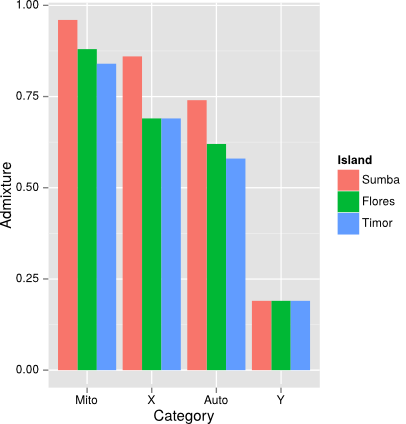
\includegraphics[width=0.85\textwidth]{../data/lansing-modified.png}
    \caption{Data from Lansing et al. [2011]. \textit{Journal of
Anthropological Archaeology}}
  \end{figure}

  \column{0.5\textwidth}
  \begin{itemize}
    \item Difference of admixture by category of DNA
    \item Sex-biased admixture
    \item Implicit marriage rule?
    \item Melanesian~\mars{} --- Asian~\female{} marriages favoured?
  \end{itemize}

\end{columns}
\end{frame}

\begin{frame}{}{Previous papers}
Questions:
\begin{itemize}
  \item Why the steep admixture gradient?
  \item Why the sex-biased admixture?
  \item What differences between the populations?
\end{itemize}
\vspace*{2em}
First step towards understanding $\rightarrow$ reproduce the scenario
\end{frame}

\subsection{Model}
\masseyBrand{}{../data/ISEA-node-map.png}{}{}
\begin{frame}{}{Model}
\vspace*{-0.8cm}
\begin{columns}
  \column{0.65\textwidth}

  \column{0.52\textwidth}
  \color{masseyWhite}
  \begin{itemize}
    \item Agent-Based Model
    \item Written in Java (Repast)
    \item Nodes $\rightarrow$ demes ($\simeq$ villages)
    \item Edges $\rightarrow$ migration paths
    \item Agent $\rightarrow$ individual or couple
  \end{itemize}

\end{columns}
\end{frame}

\masseyBrand{}{../data/ISEA-node-map.png}{}{}
\begin{frame}{}{Model}
\vspace*{-0.8cm}
\begin{columns}
  \column{0.65\textwidth}

  \column{0.52\textwidth}
  \color{masseyWhite}
  My goals:
  \begin{itemize}
    \item Assess the quality of the model
    \item Compare the results to the real data (reference)
    \item Provide a statistical framework to analyse the results
  \end{itemize}

\end{columns}
\end{frame}


\section{Measures and comparisons}
\masseyBrand{bar}[0.1]{}{}{}
\begin{frame}{}{Table of contents}
\tableofcontents[currentsection, subsectionstyle=show/show/hide, subsubsectionstyle=show/show/show/shaded]
\end{frame}

\subsection{Observed data}
\begin{frame}{Measures \& comparisons}{Observed data}
\begin{columns}
  \column{0.6\textwidth}
  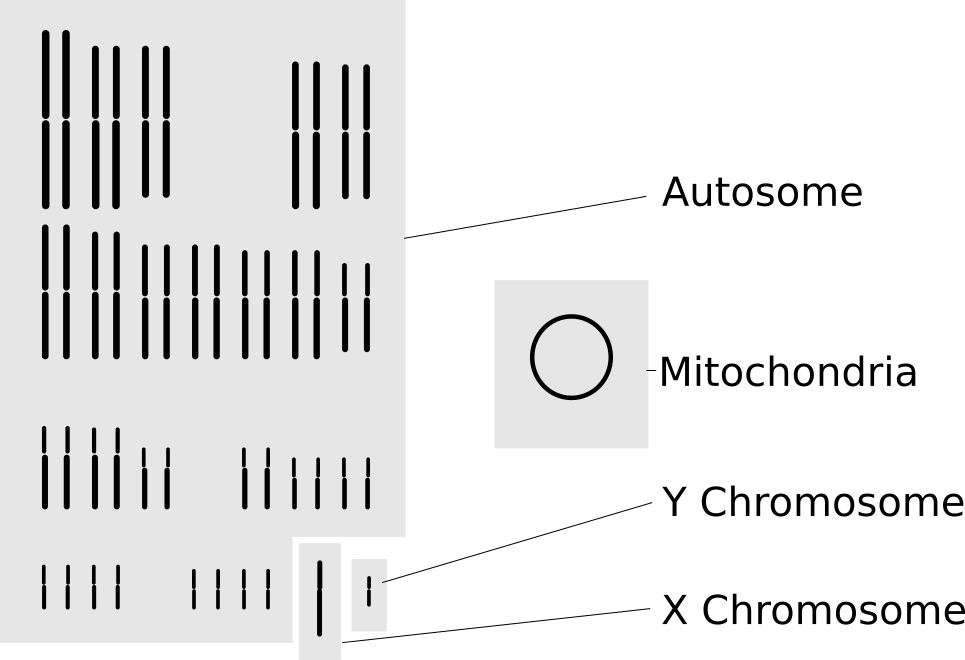
\includegraphics[width=1\textwidth]{../data/markers.png}

  \column{0.5\textwidth}
  \begin{itemize}
    \item Discriminant markers
    \item Different parts of the DNA
    \item Associated with different origins
    \item Inside the model: values by agent
    \item Output of the model: values by deme
  \end{itemize}

\end{columns}
\end{frame}

\subsection{Parameters}
\begin{frame}{Measures \& comparisons}{Parameters}
\begin{table}[H]
	\hspace*{-0.5cm}
	\begin{tabu}{@{}l>{\footnotesize}ll@{}}
	  \toprule
 	  Parameter & \normalsize Estimated & Comment \\
 	  \midrule
    Migration prob. & $0.0 < x \leq 1.0$ & for a Melanesian agent \\
    Migration prob. ratio & $1.0 \leq x \leq 4.0$ & corresponding ratio for an Asian agent \\
    Fecundity & $2.5 < x < 8.0$ & for a Melanesian agent \\
    Fecundity ratio & $1.0 \leq x \leq 2.0$ & corresponding ratio for an Asian agent \\
    Marriage threshold & $0.0 \leq x \leq 0.25$ & affects marriages rules \\
	  \rowfont{\color{gray}}
    Growth rate & $0.0 < x < 0.001$ & limiting rate of pop. growth \\
	  \rowfont{\color{gray}}
    Number of agents & $100 \leq x < 400$ & pop. size in each deme, initially \\
	  \rowfont{\color{gray}}
    Graph & \{...\} & nodes and edges of the graph \\
	  \rowfont{\color{gray}}
    Starting distribution & \{...\} & distribution of pop. in the graph \\ 
    \bottomrule
	\end{tabu}
	\caption{Summary of the changing model parameters.}
\end{table}
\end{frame}

\subsection{Comparison functions}
\begin{frame}{Measures \& comparisons}{Comparison functions}
\begin{center}
  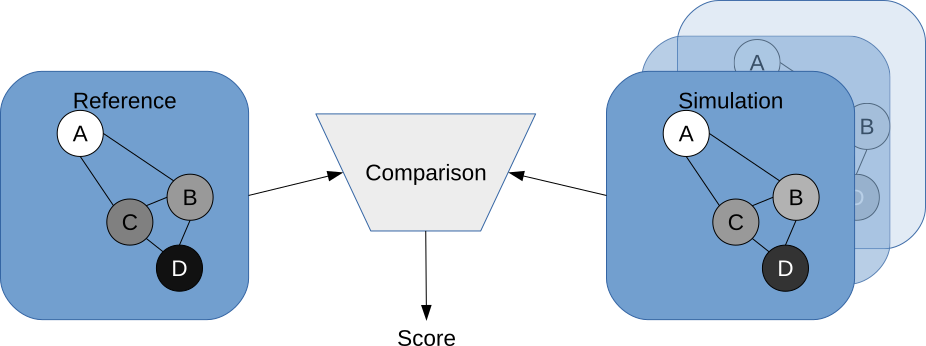
\includegraphics[width=1\textwidth]{../data/comparison-general.png}
\end{center}
\end{frame}

\subsubsection{Mean Square Distance}
\begin{frame}{Measures \& comparisons}{Comparison functions}
\begin{mblock}{0.7}{Mean Square Distance}
  \centering  
  $\mathit{MSD} = \frac{\sum\limits_{i=1}^{n} \left( AdRef_i - AdSim_i \right) ^ 2}{n}$\\~\\
  $0 \le \mathit{MSD} \le 1$
\end{mblock}
\pause
\begin{mblock}{0.7}{Example}
  \begin{center}
    \begin{tabu}{@{}lcccc@{}}
      \toprule[1pt]
      Island & A & B & C & D \\
      \midrule
      Reference & 1.0 & 0.5 & 0.4 & 0.0 \\
      Simulated & 1.0 & 0.4 & 0.3 & 0.2 \\
      Distance$^2$ & 0.0 & 0.01 & 0.01 & 0.04 \\
      \bottomrule[1pt]
    \end{tabu}
  \end{center}
  \centering
  $\mathit{MSD} = 0.015$
\end{mblock}
\end{frame}

\subsubsection{Partial Mantel Correlation}
\begin{frame}{Measures \& comparisons}{Comparison functions}
\begin{mblock}{0.7}{Mantel Partial Correlation}
  \centering  
  $cor = mantel.partial \left( M_{Simulated}, M_{Reference}, M_{geographical} \right)\ $\\~\\
  $-1 \le cor \le 1$
\end{mblock}
\pause
\begin{mblock}{0.7}{Example}
  \begin{center}
    \hspace*{-0.5cm}
    \fontsize{5.5pt}{8pt}
    $mantel.partial \left( \begin{bmatrix}
      0.0 & 0.5 & 0.6 & 1.0 \\
      0.5 & 0.0 & 0.1 & 0.5 \\
      0.6 & 0.1 & 0.0 & 0.4 \\
      1.0 & 0.5 & 0.4 & 0.0 \\
    \end{bmatrix}, \begin{bmatrix}
      0.0 & 0.6 & 0.7 & 0.8 \\
      0.6 & 0.0 & 0.1 & 0.2 \\
      0.7 & 0.1 & 0.0 & 0.1 \\
      0.8 & 0.2 & 0.1 & 0.0 \\
    \end{bmatrix}, \begin{bmatrix}
      0.0 & 300 & 250 & 400 \\
      300 & 0.0 & 120 & 150 \\
      250 & 120 & 0.0 & 100 \\
      400 & 150 & 100 & 0.0 \\
    \end{bmatrix} \right) $
  \end{center}
  \centering
  $cor = 0.72$
\end{mblock}
\end{frame}

\subsubsection{Summary statistics}
\begin{frame}{Measures \& comparisons}{Comparison functions}
Summary statistics:
\begin{itemize}
  \item Mean Square Distance
  \begin{itemize}
    \item Autosomal admixture
    \item X-Chromosomal admixture
  \end{itemize}
  \item Partial Mantel Correlation
  \begin{itemize}
    \item Autosomal admixture
    \item X-Chromosomal admixture
  \end{itemize}
\end{itemize}
\end{frame}


\section{Pipeline}
\begin{frame}{}{Table of contents}
\tableofcontents[currentsection, subsectionstyle=show/show/hide]
\end{frame}

\subsection{Overview}
\begin{frame}{Pipeline}{Overview}
\begin{center}
  \begin{tikzpicture}
    \node[anchor=south west, inner sep=0] at (0, 0) {
      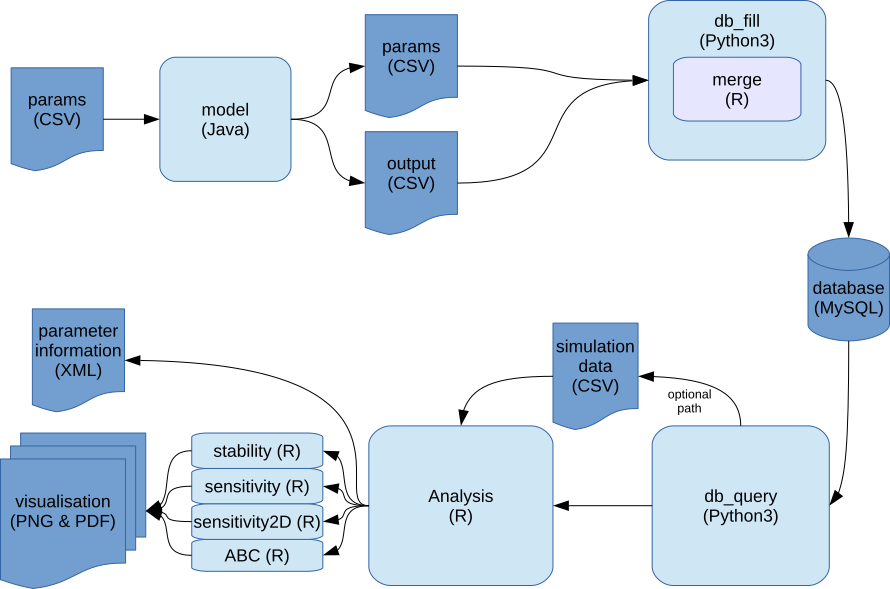
\includegraphics[width=1\textheight]{../data/workflow-2.png}
    };
  \end{tikzpicture}
\end{center}
\end{frame}

\addtocounter{framenumber}{-1}
\begin{frame}{Pipeline}{Model runs}
\begin{center}
  \begin{tikzpicture}
    \node[anchor=south west, inner sep=0] at (0, 0) {
      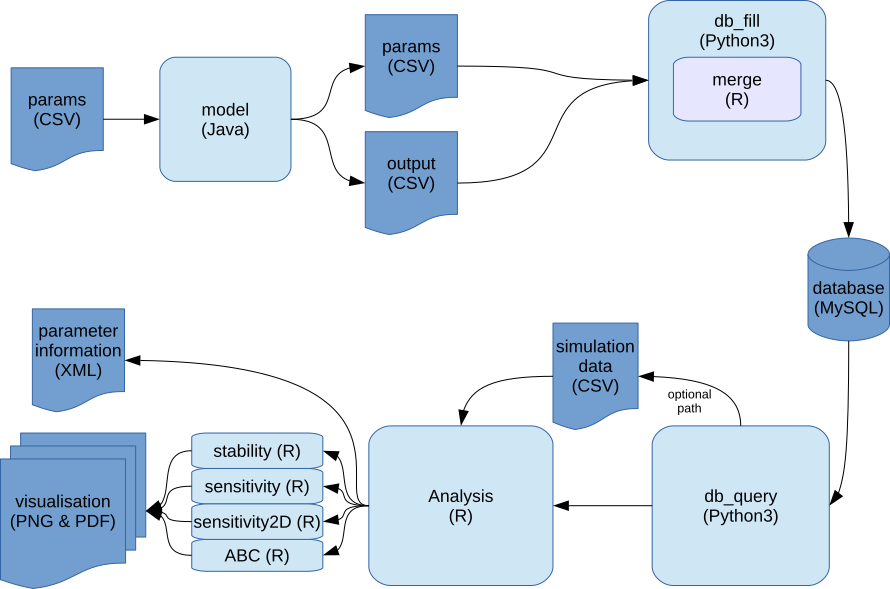
\includegraphics[width=1\textheight]{../data/workflow-2.png}
    };
    \draw[masseyGold, ultra thick, rounded corners] (0, 3.5) rectangle (5, 6.1);
  \end{tikzpicture}
\end{center}
\end{frame}

\addtocounter{framenumber}{-1}
\begin{frame}{Pipeline}{Data merging, aggregating and storage}
\begin{center}
  \begin{tikzpicture}
    \node[anchor=south west, inner sep=0] at (0, 0) {
      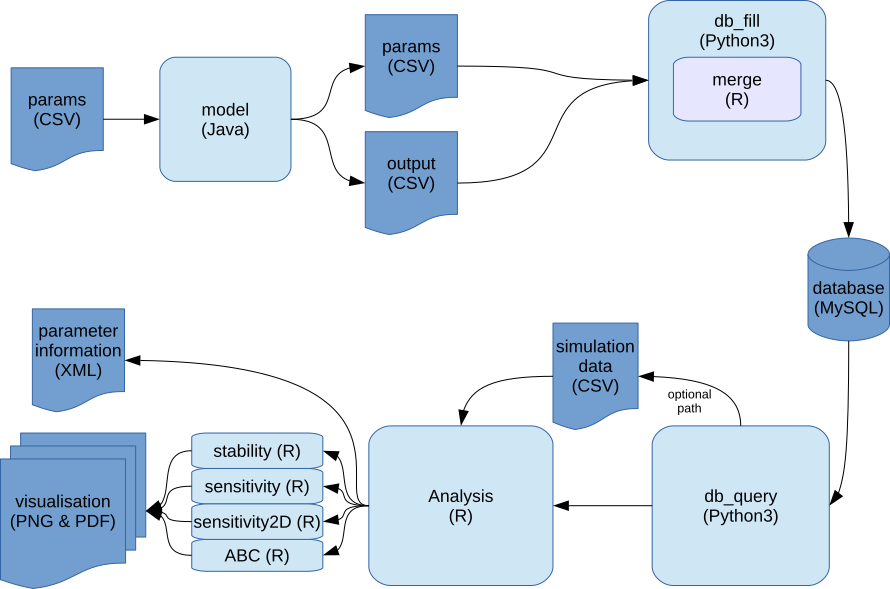
\includegraphics[width=1\textheight]{../data/workflow-2.png}
    };
    \draw[masseyGold, ultra thick, rounded corners] (3.3, 2.5) rectangle (9.2, 6.2);
  \end{tikzpicture}
\end{center}
\end{frame}

\addtocounter{framenumber}{-1}
\begin{frame}{Pipeline}{Data querying}
\begin{center}
  \begin{tikzpicture}
    \node[anchor=south west, inner sep=0] at (0, 0) {
      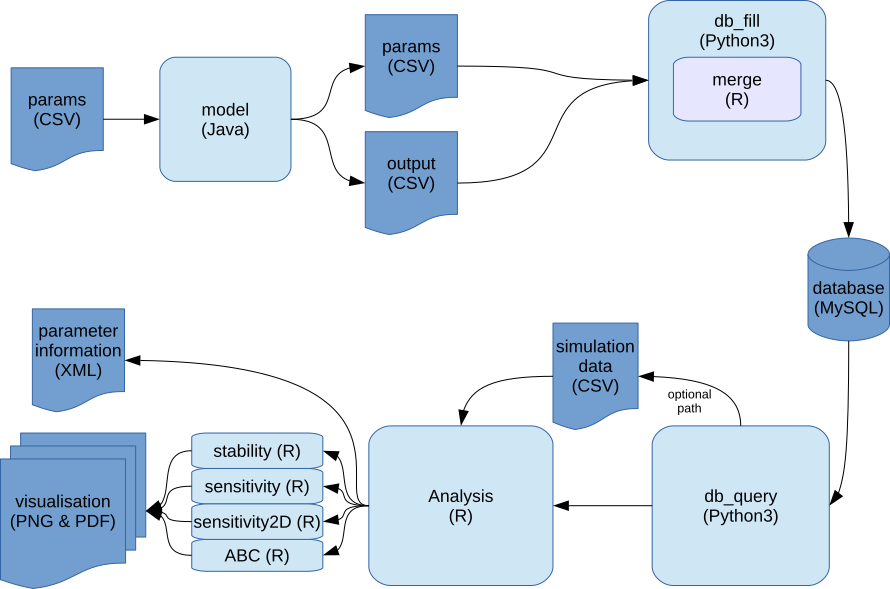
\includegraphics[width=1\textheight]{../data/workflow-2.png}
    };
    \draw[masseyGold, ultra thick, rounded corners] (5.5, 0) rectangle (9.2, 3.8);
  \end{tikzpicture}
\end{center}
\end{frame}

\addtocounter{framenumber}{-1}
\begin{frame}{Pipeline}{Analyses}
\begin{center}
  \begin{tikzpicture}
    \node[anchor=south west, inner sep=0] at (0, 0) {
      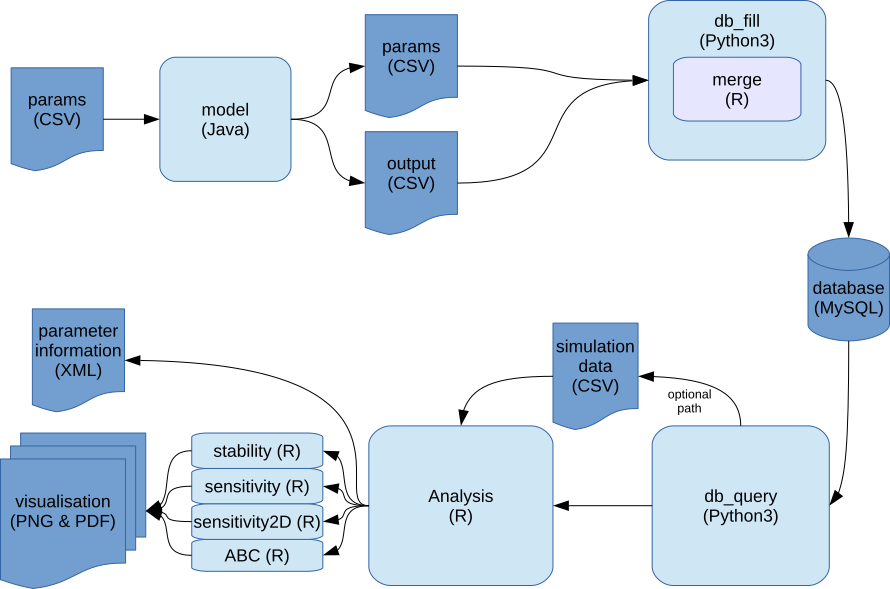
\includegraphics[width=1\textheight]{../data/workflow-2.png}
    };
    \draw[masseyGold, ultra thick, rounded corners] (0, 0) rectangle (6.8, 3.2);
  \end{tikzpicture}
\end{center}
\end{frame}

\addtocounter{framenumber}{-1}
\begin{frame}{Pipeline}{Overview}
\begin{center}
  \begin{tikzpicture}
    \node[anchor=south west, inner sep=0] at (0, 0) {
      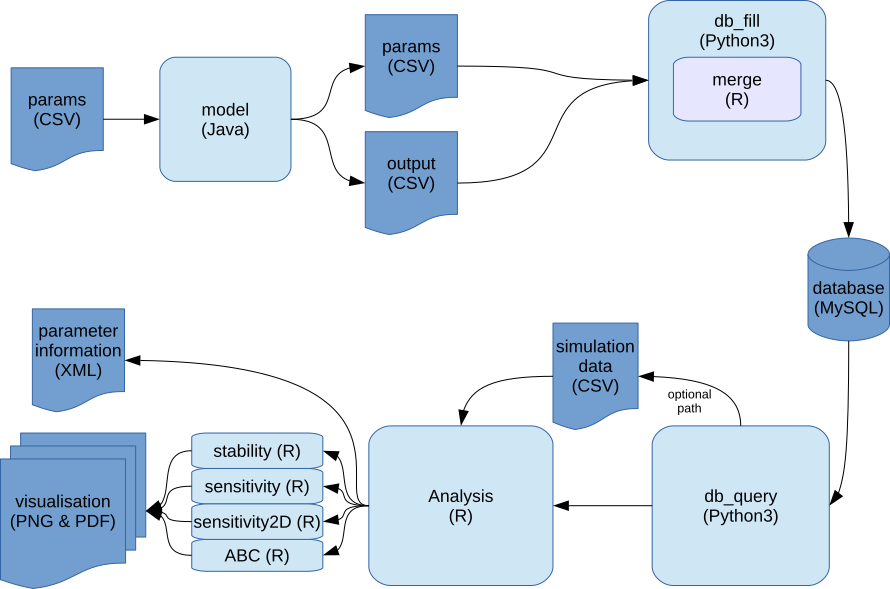
\includegraphics[width=1\textheight]{../data/workflow-2.png}
    };
  \end{tikzpicture}
\end{center}
\end{frame}


\section{Statistical analysis}
\begin{frame}{}{Table of contents}
\tableofcontents[currentsection, subsectionstyle=show/show/hide]
\end{frame}

\subsection{Grid search}
\begin{frame}{Statistical analysis}{Grid search}
\begin{center}
  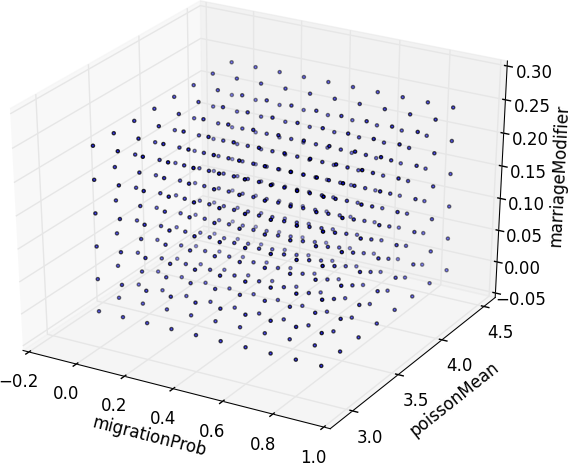
\includegraphics[width=0.8\textwidth]{../data/grid.png}
\end{center}
\end{frame}

\begin{frame}{Statistical analysis}{Grid search}
\begin{center}
  \begin{figure}
    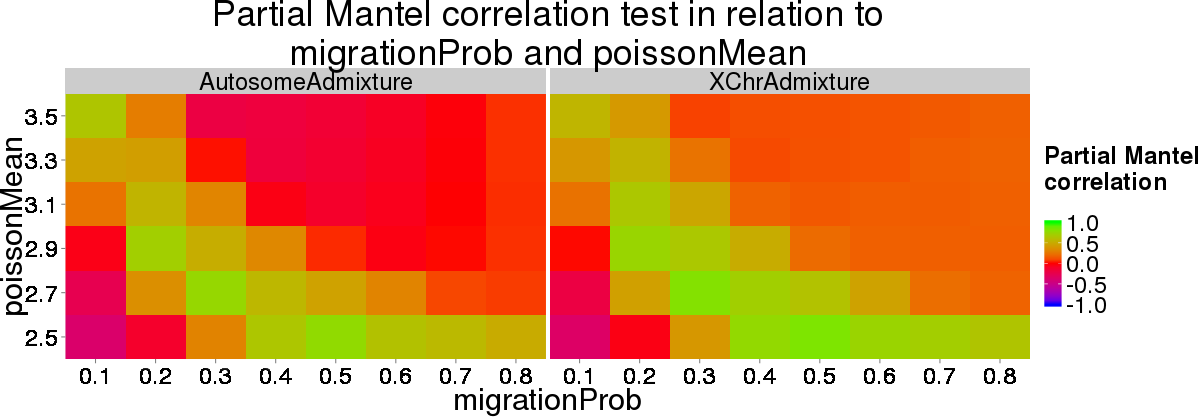
\includegraphics[width=1\textwidth]{../data/sensit-comp-2d-preview.png}
  \end{figure}
\end{center}
\end{frame}

\subsection{Approximate Bayesian Computation}
\begin{frame}{Statistical analysis}{Approximate Bayesian Computation}
\begin{center}
  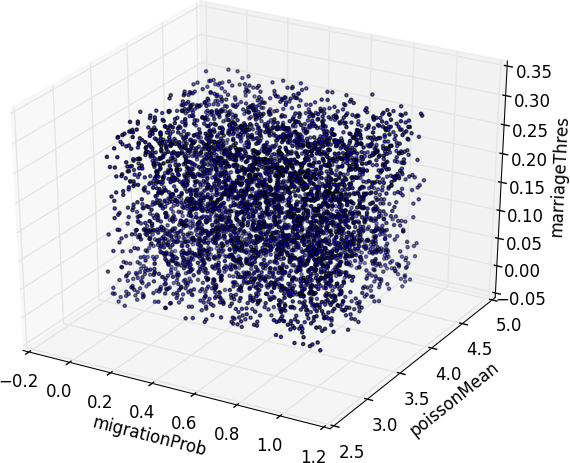
\includegraphics[width=0.8\textwidth]{../data/abc-space.png}
\end{center}
\end{frame}

\begin{frame}{Statistical analysis}{Approximate Bayesian Computation}
\begin{center}
  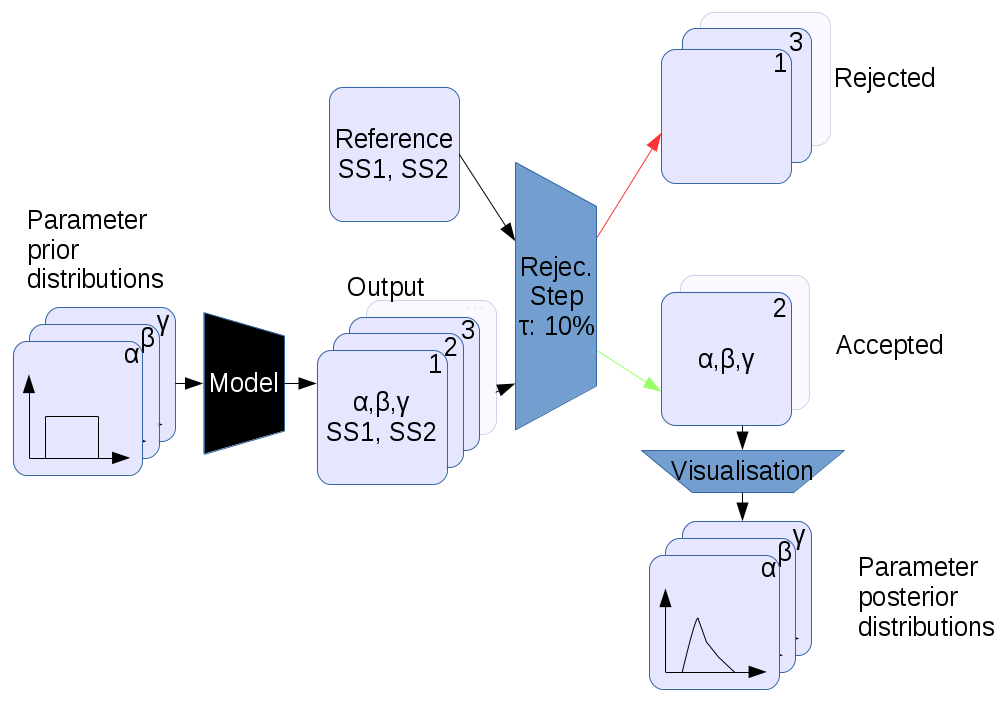
\includegraphics[width=0.94\textwidth]{../data/abc-landscape.png}
\end{center}
\end{frame}

\begin{frame}{Statistical analysis}{Approximate Bayesian Computation}
\begin{center}
  \begin{figure}
    \hspace*{-0.85cm}
    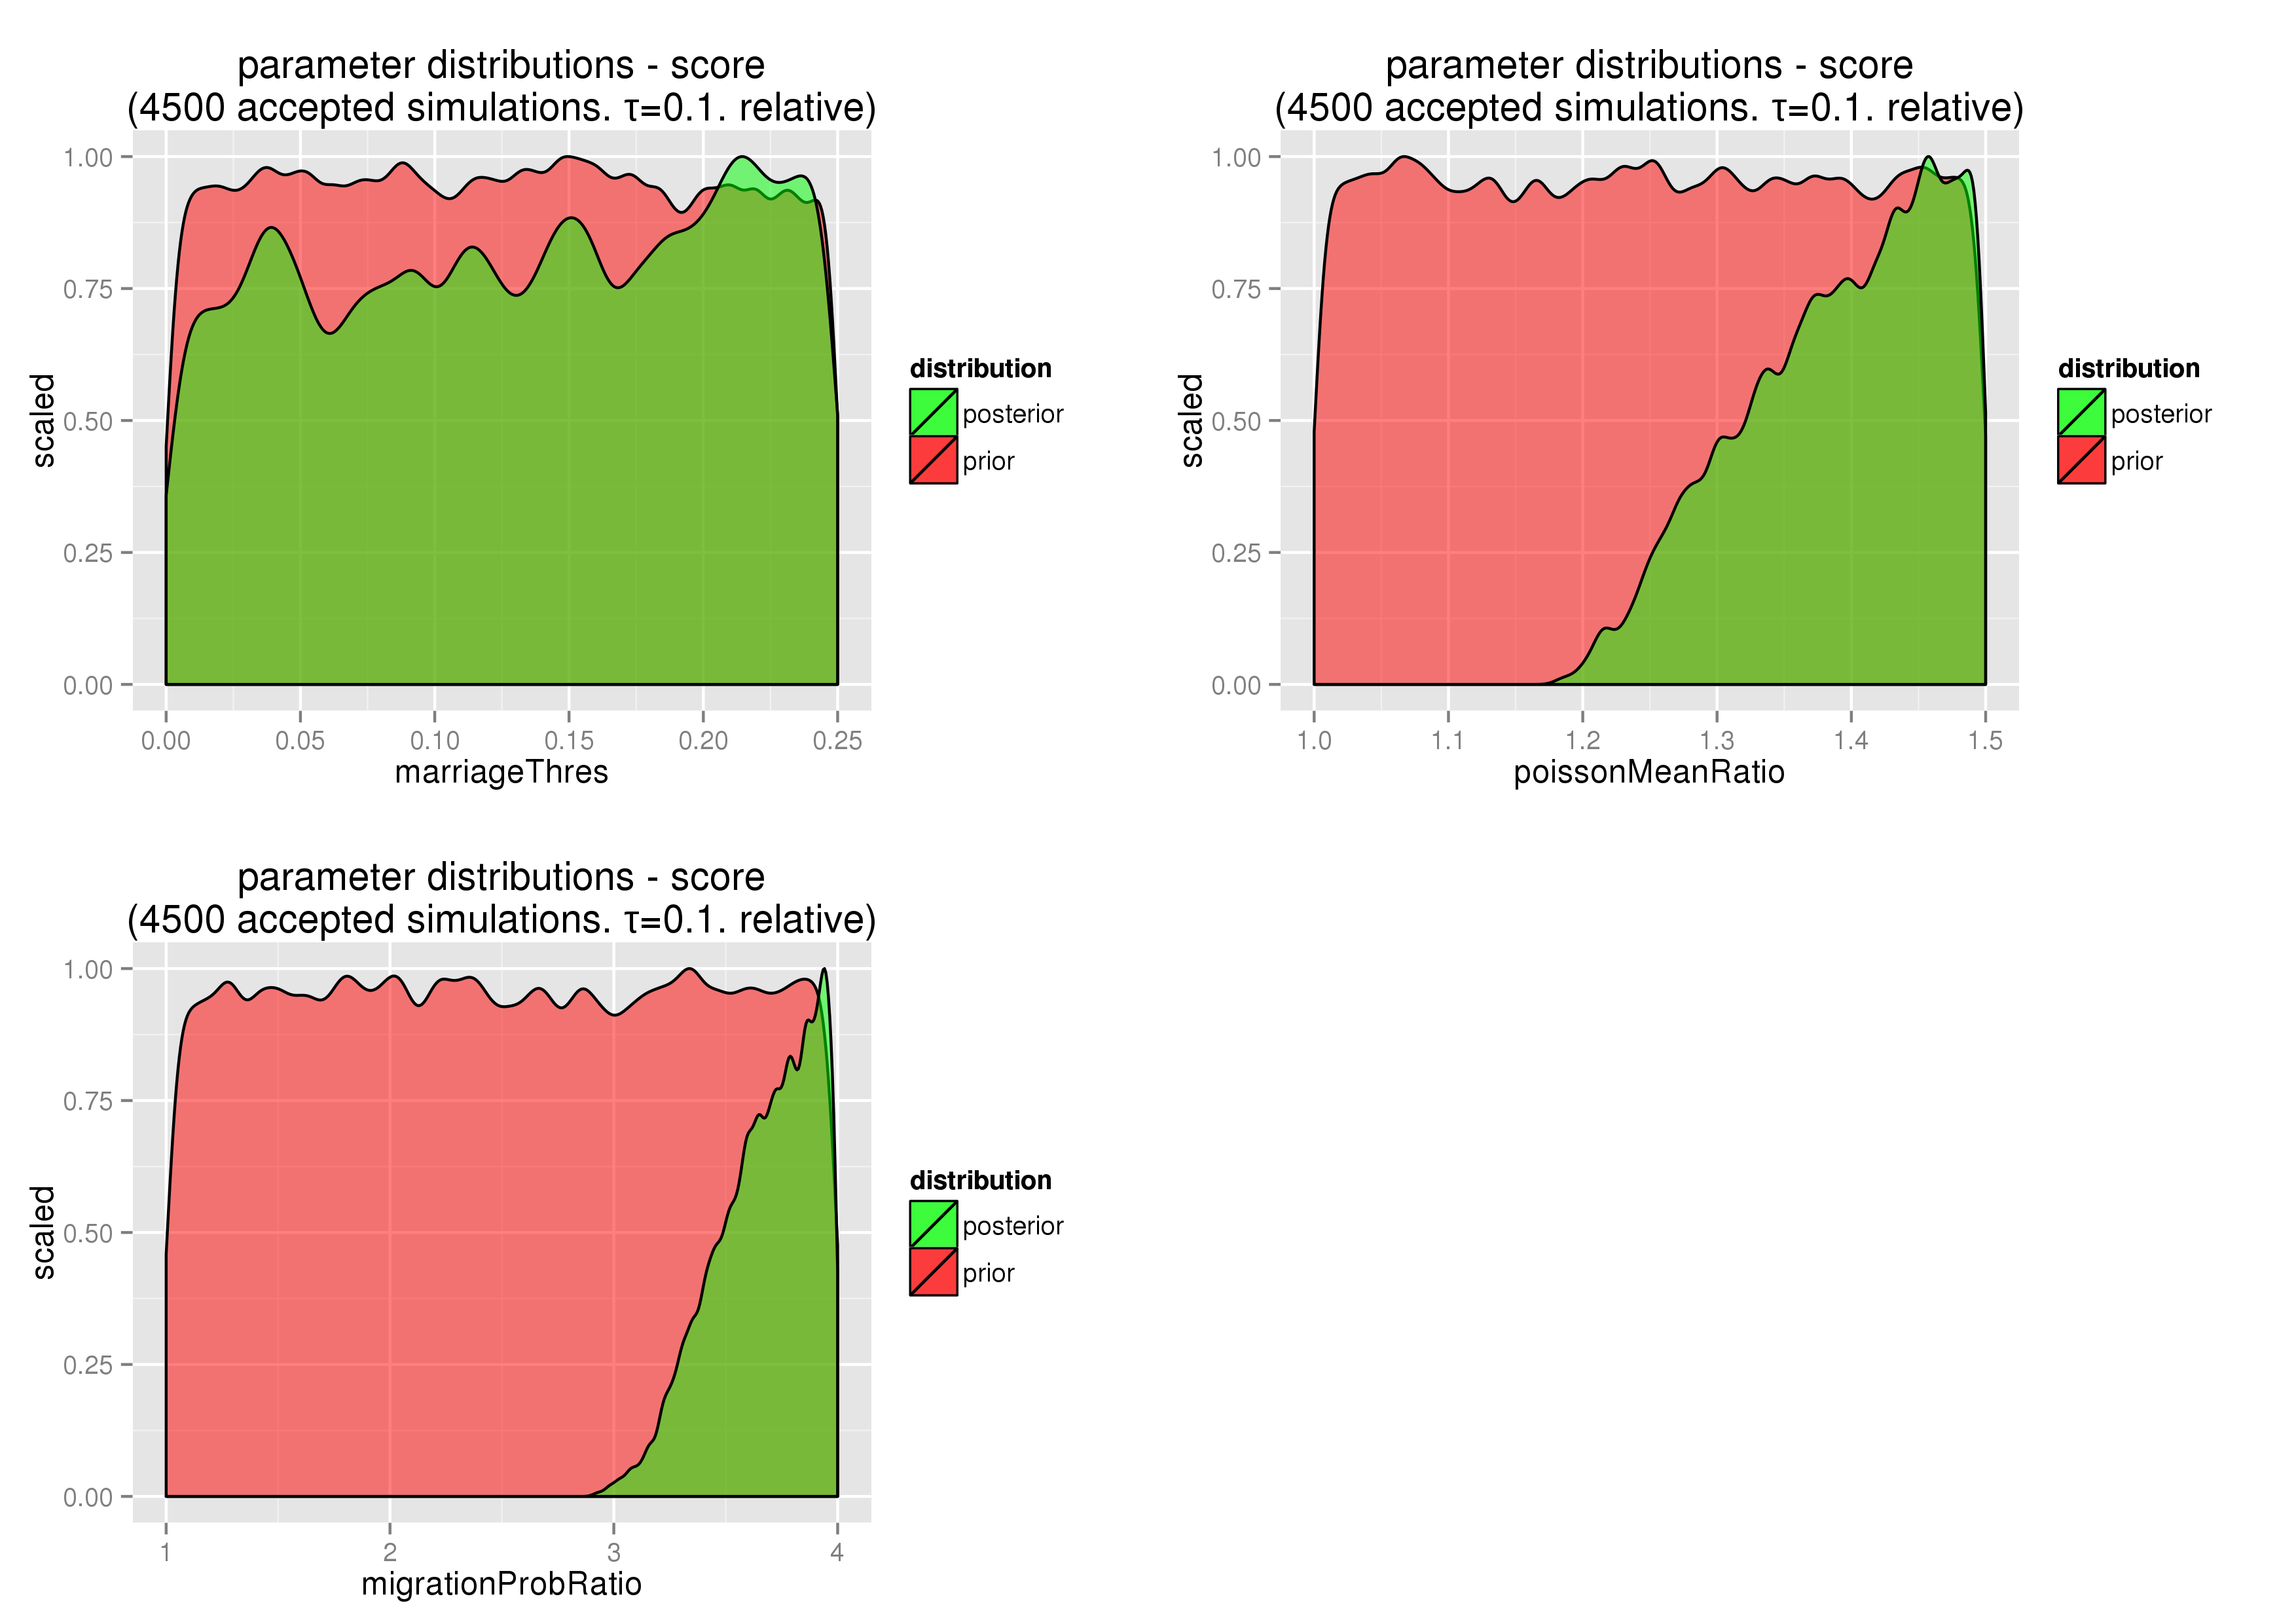
\includegraphics[width=1.15\textwidth]{../data/abc-priors-posteriors.png}
    \caption{Example output from an ABC analysis}
  \end{figure}
\end{center}
\end{frame}

\section*{Conclusion}
\begin{frame}{}{Conclusion}
\begin{columns}
  \column{0.5\textwidth}
  \begin{itemize}
    \item Pipeline:
    \begin{itemize}
      \item Modular pipeline
      \item Stream processing
      \item Database use
    \end{itemize}
  \end{itemize}
  \vspace*{1em}
  \begin{itemize}
    \item Statistically powerful approach:
    \begin{itemize}
      \item Approximate Bayesian Computation
      \item Accept good results
      \item Discard bad results
    \end{itemize}
  \end{itemize}

  \column{0.5\textwidth}
  \begin{itemize}
    \item “Austronesian Expansion”:
    \begin{itemize}
      \item Higher fecundity
      \item Higher migration rates
      \item Melanesian~\mars{} --- Asian~\female{} marriages favoured
    \end{itemize}
  \end{itemize}

\end{columns}
\end{frame}

% Closing ------------------------------------------------------------------------------------

\begin{frame}[plain]
\masseyClose{Thank you}
%\begin{columns}
  %\column{0.58\textwidth}
    %\tableofcontents[subsubsectionstyle=hide]

  %\column{0.56\textwidth}
    \color{masseyBlue}
    \begin{Huge}
      Questions?
    \end{Huge}
    \\~\\~\\~\\~\\
    \begin{small}
      \color{gray}
      map backgrounds from “HERE Satellite”
    \end{small}
    \\~\\
    Computational Biology Research Group: \href{http://massey.genomicus.com}{\texttt{massey.genomicus.com}}

%\end{columns}
\end{frame}

% Appendices

\masseyBrand{full}{uniLogo/masseyBlueCircles.jpg}{}{}
\begin{frame}[plain, noframenumbering]{}{Comparison functions}
\begin{figure}
  \hspace*{-1cm}
  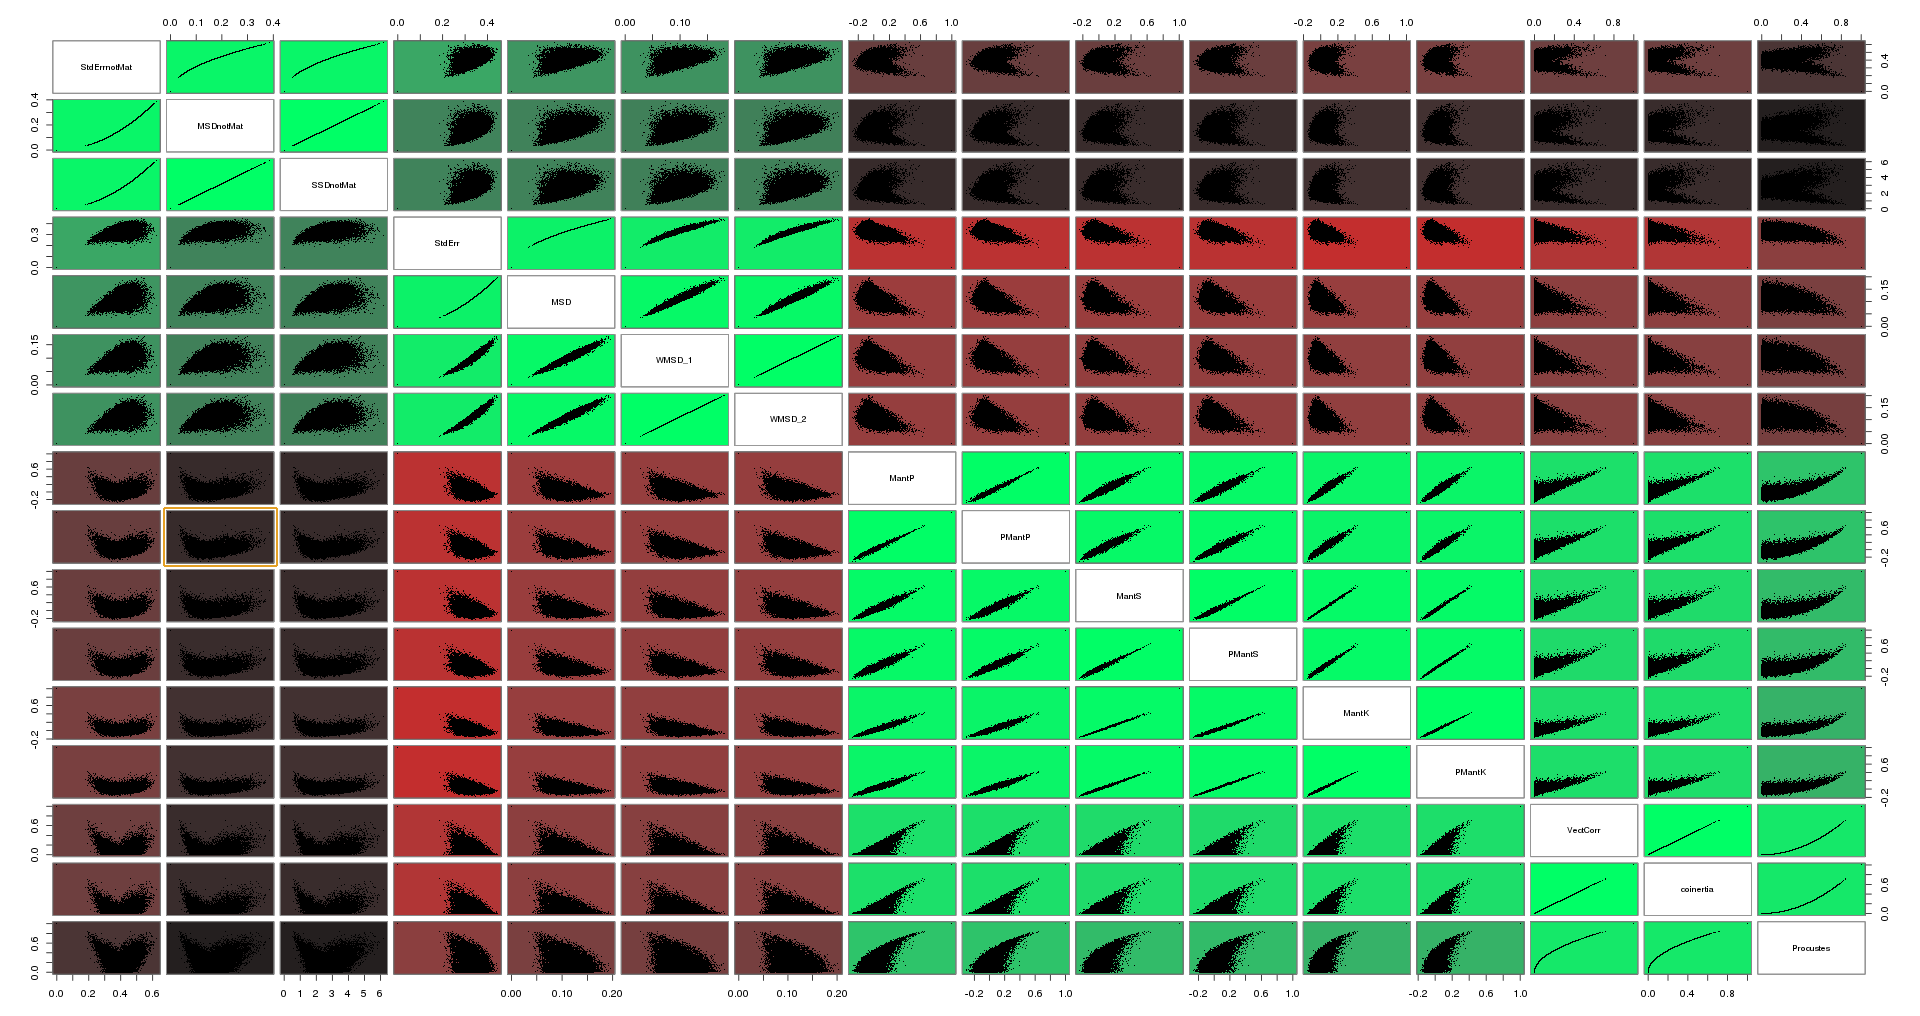
\includegraphics[width=1.17\textwidth]{../data/comparisonFunctions.png}
\end{figure}
\end{frame}

\begin{frame}[plain, noframenumbering]{}{Database structure}
\begin{figure}
  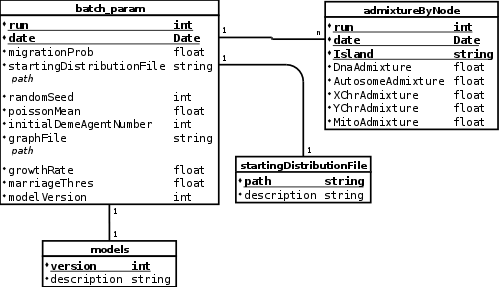
\includegraphics[width=1\textwidth]{../data/DB.png}
\end{figure}
\end{frame}

\begin{frame}[plain, noframenumbering]{}{Sensitivity 1D - comparisons}
\begin{figure}
  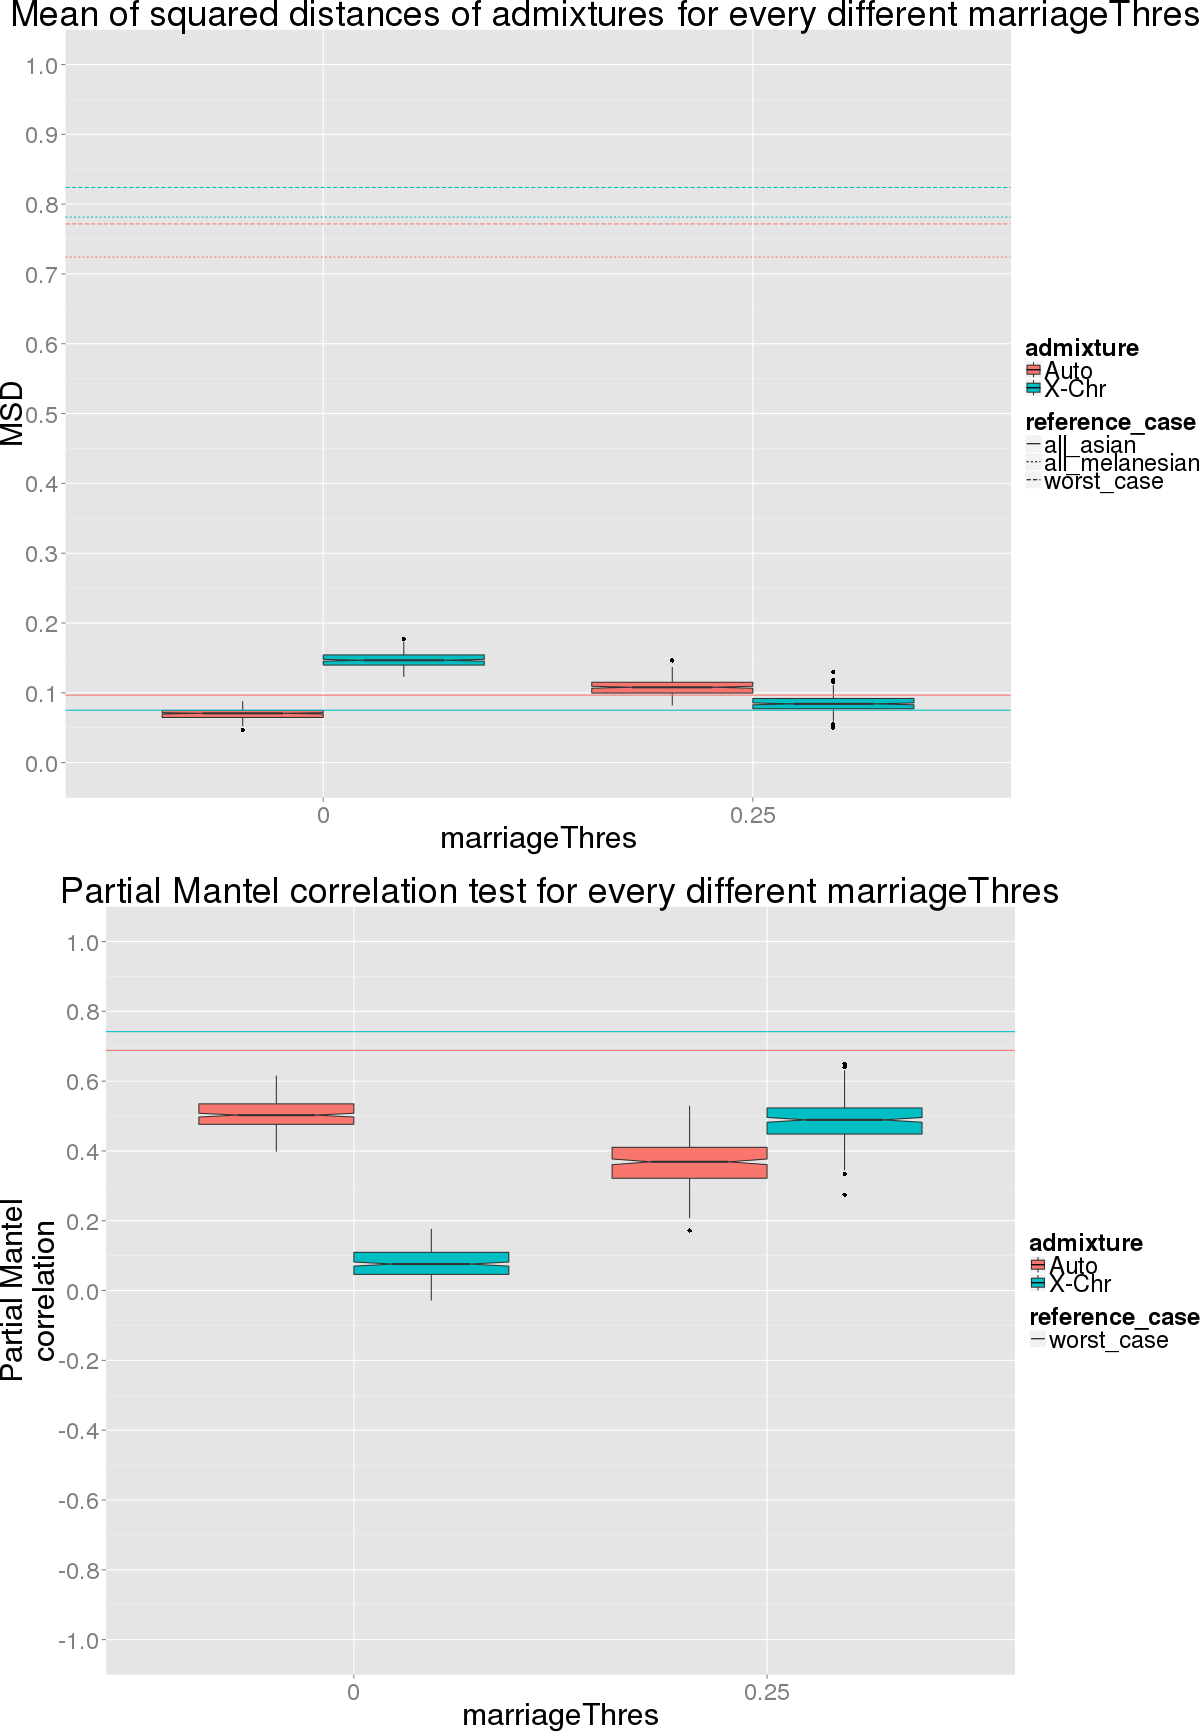
\includegraphics[width=0.48\textwidth]{../data/sensit-comp-1d.png}
\end{figure}
\end{frame}

\begin{frame}[plain, noframenumbering]{}{Sensitivity 2D - comparisons}
\begin{figure}
  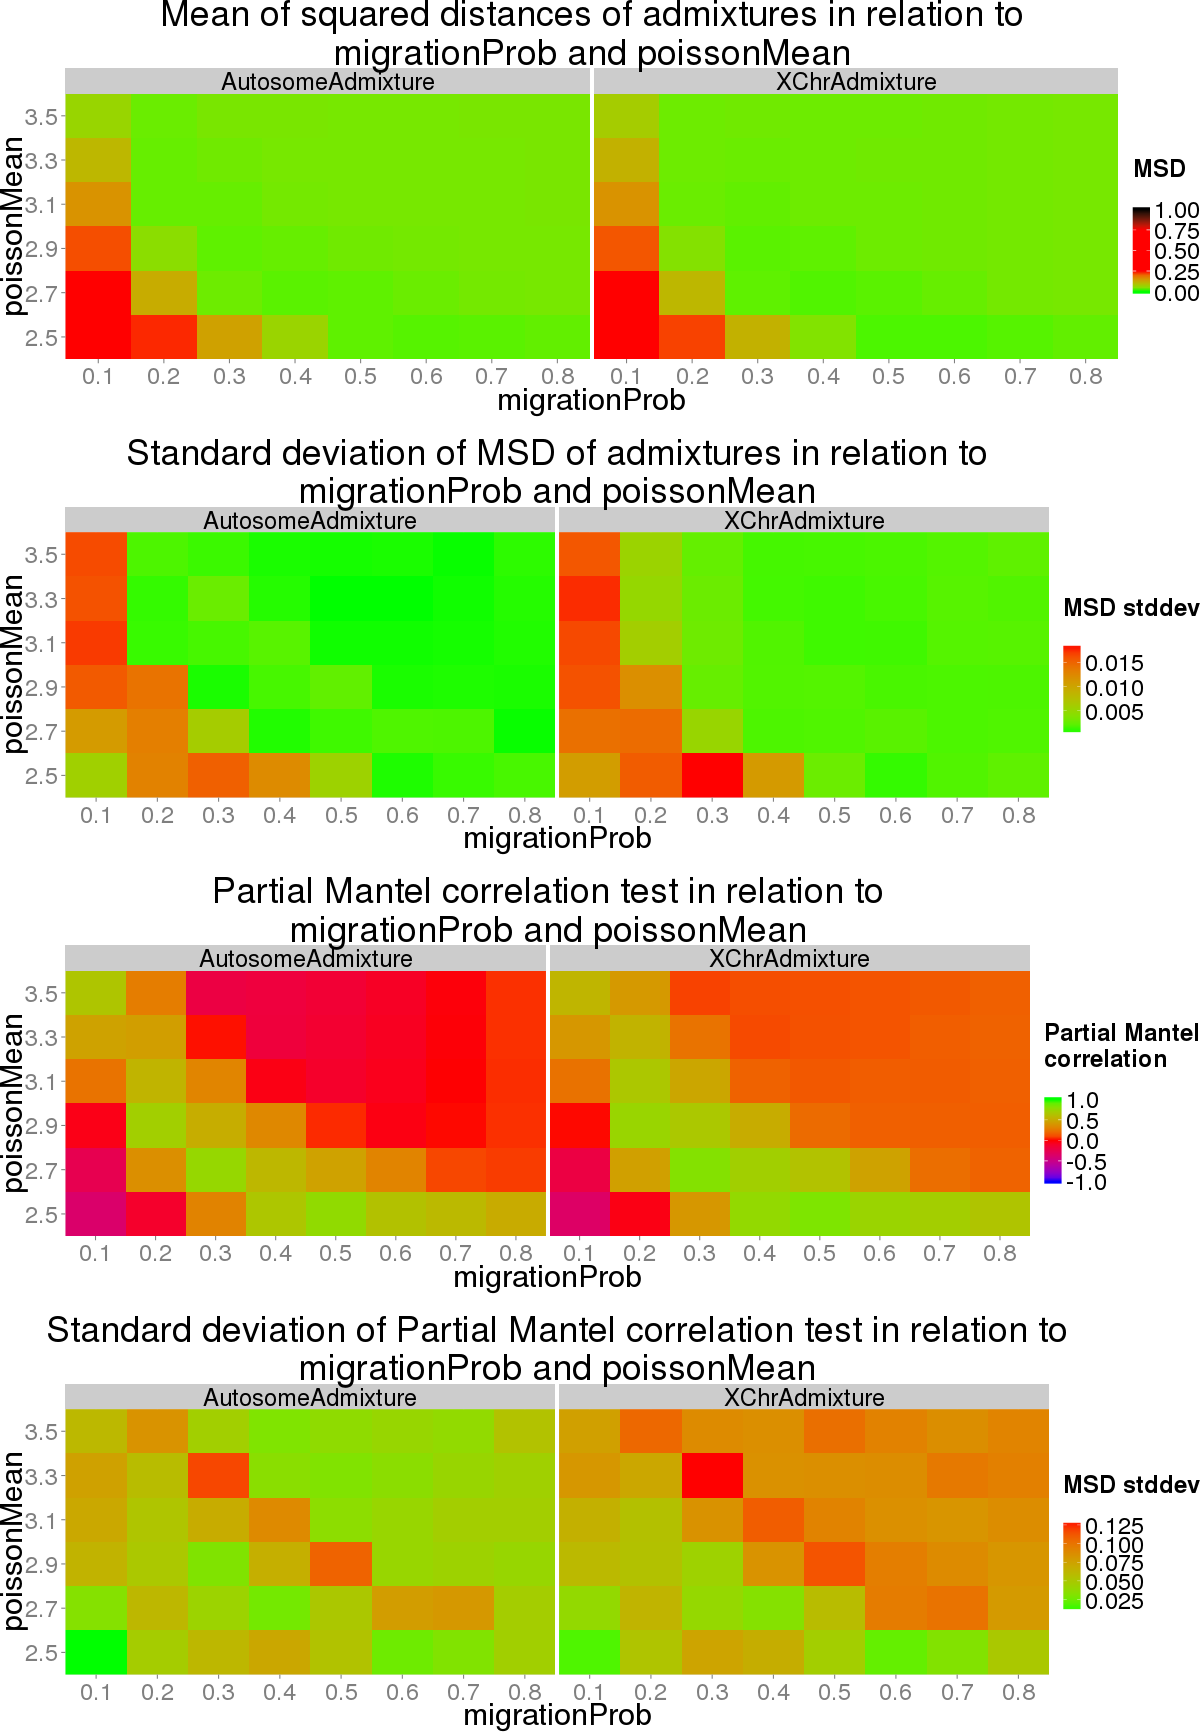
\includegraphics[width=0.48\textwidth]{../data/sensit-comp-2d.png}
\end{figure}
\end{frame}

\begin{frame}[plain, noframenumbering]{}{ABC scatter score}
\begin{figure}
  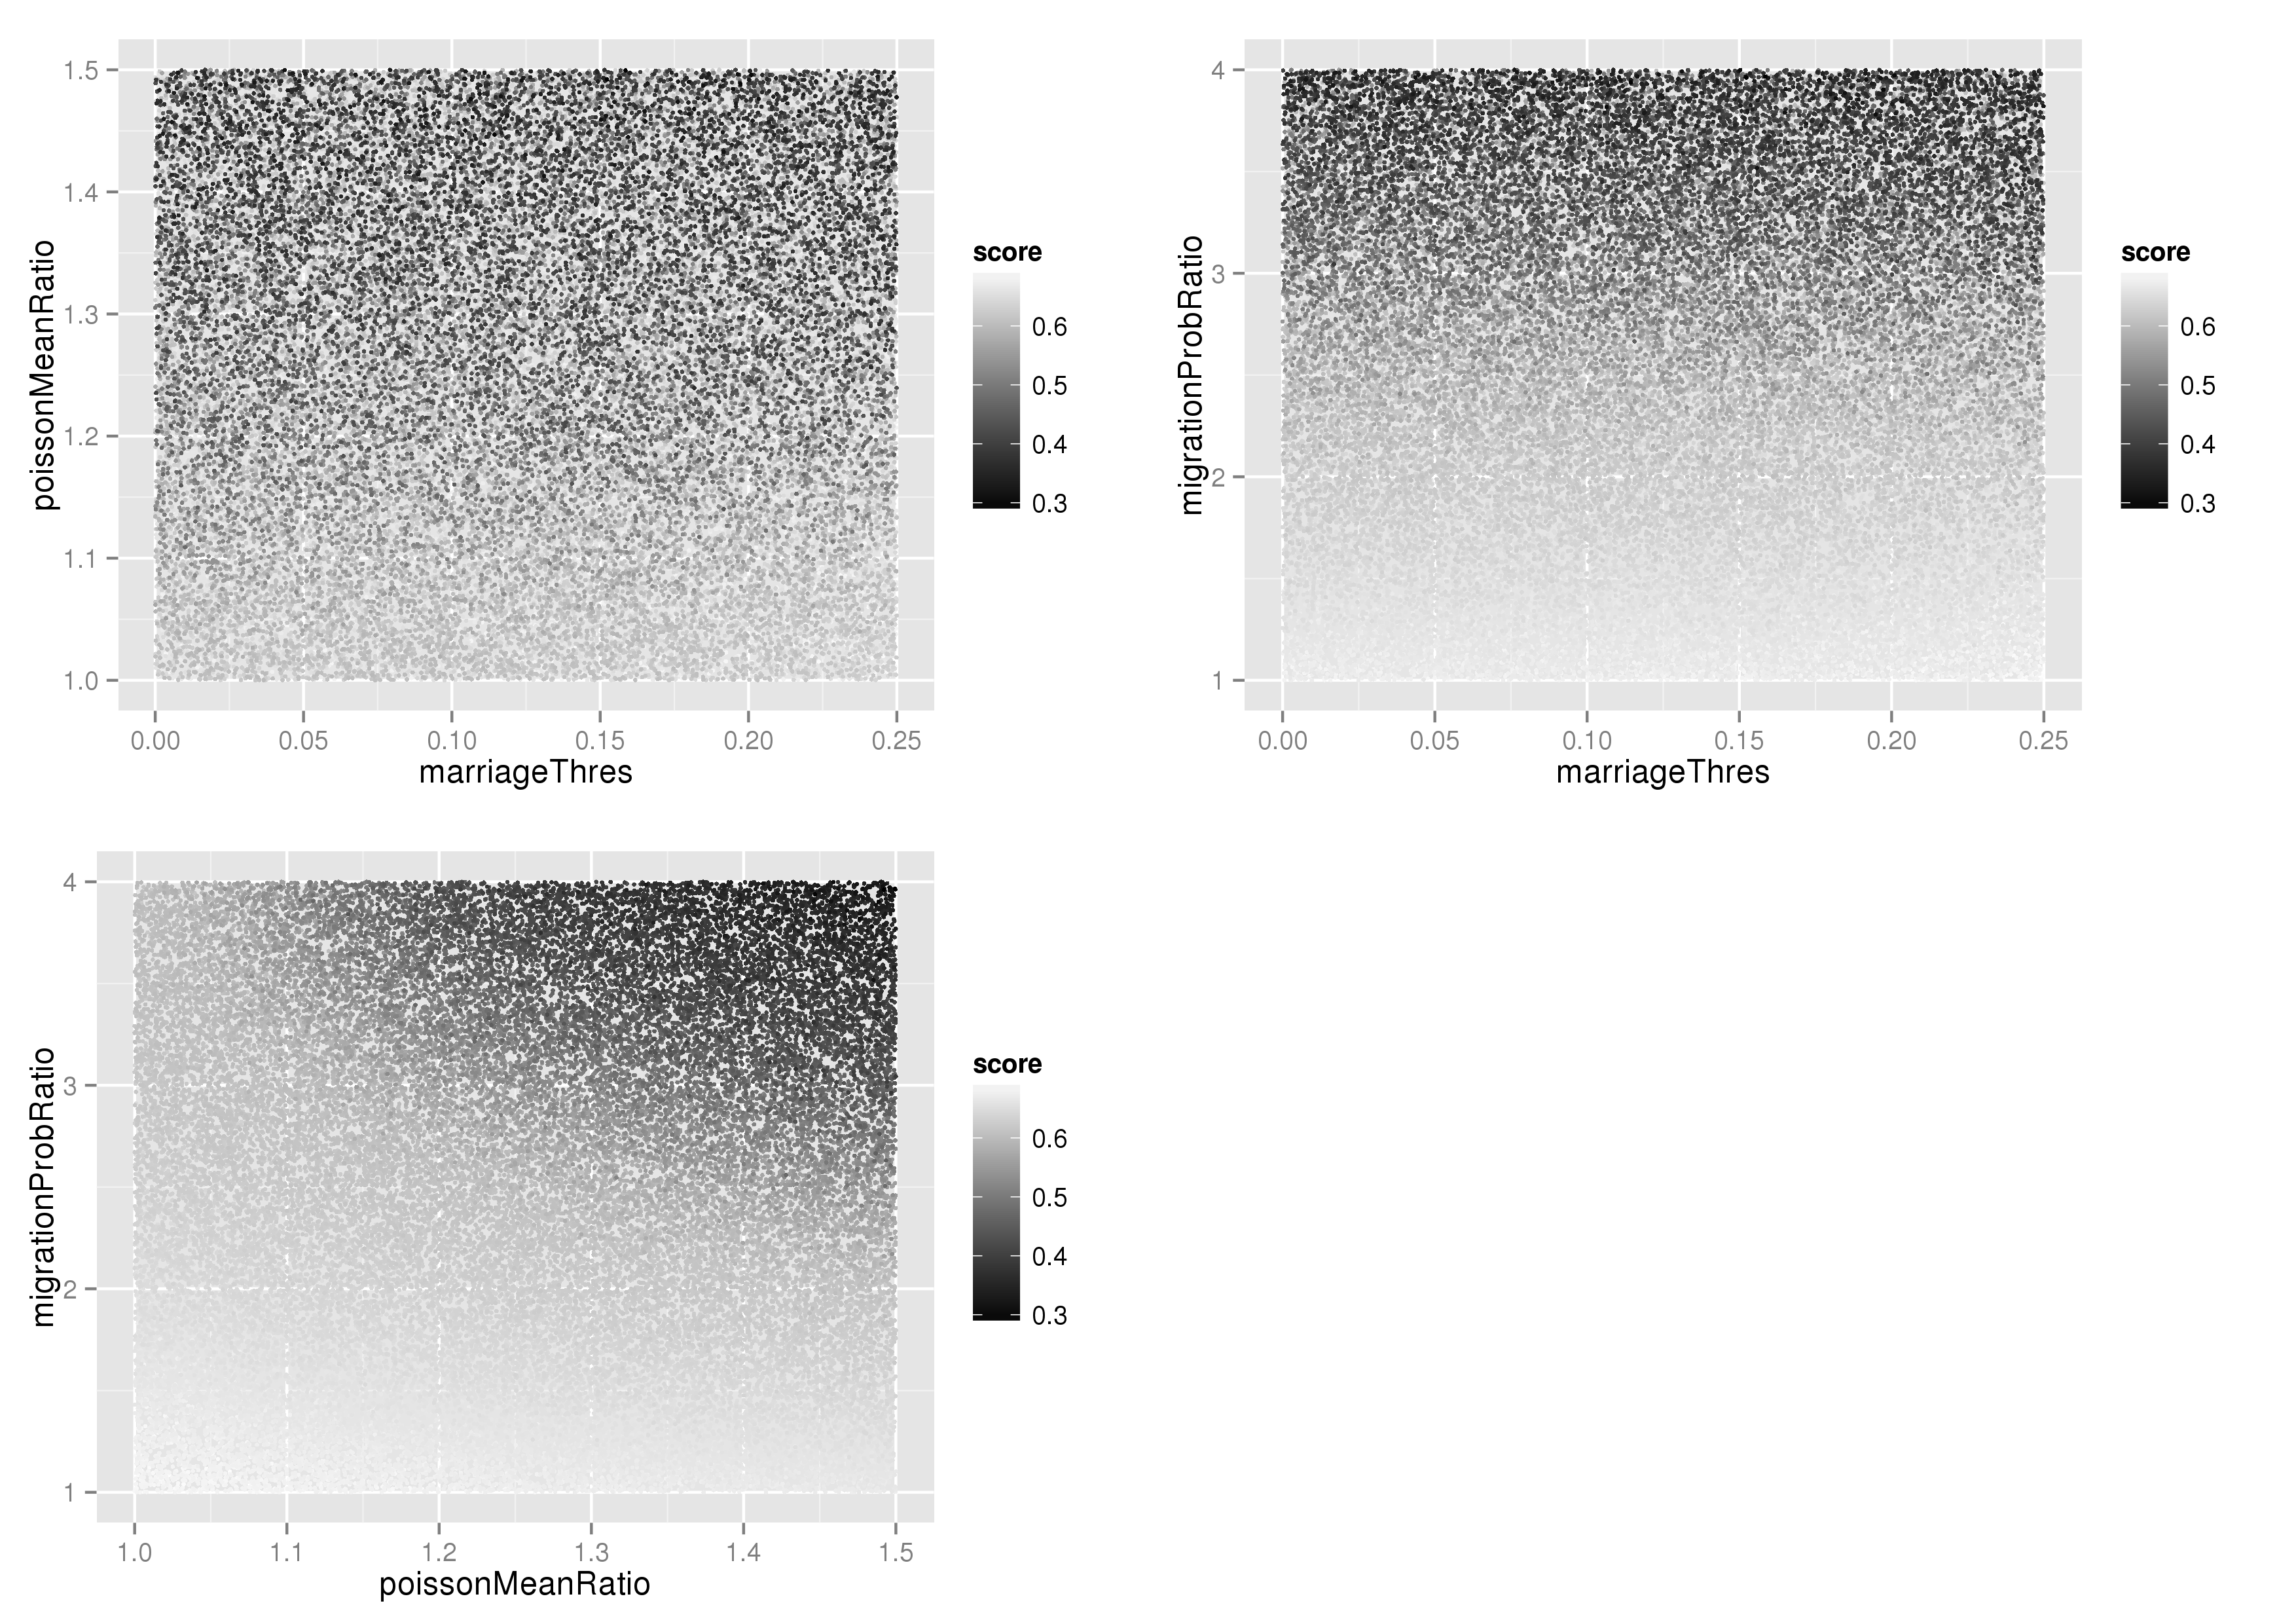
\includegraphics[width=0.9\textwidth]{../data/abc-scatter-score.png}
\end{figure}
\end{frame}

\begin{frame}[plain, noframenumbering]{}{Benchmark \texttt{merge}}
\begin{figure}
  \hspace*{-1cm}
  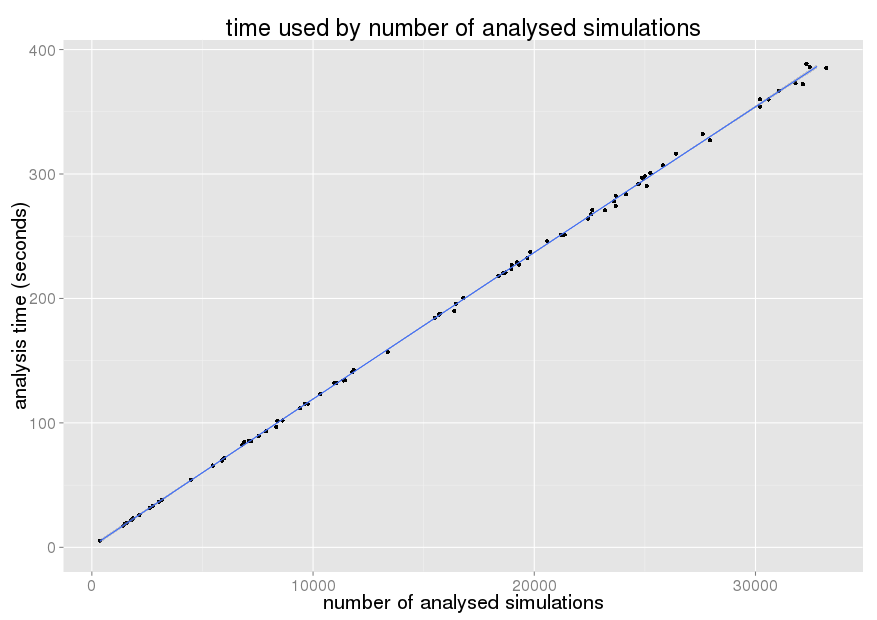
\includegraphics[width=0.585\textwidth]{../data/merge-timeByNSimulations.png}%
  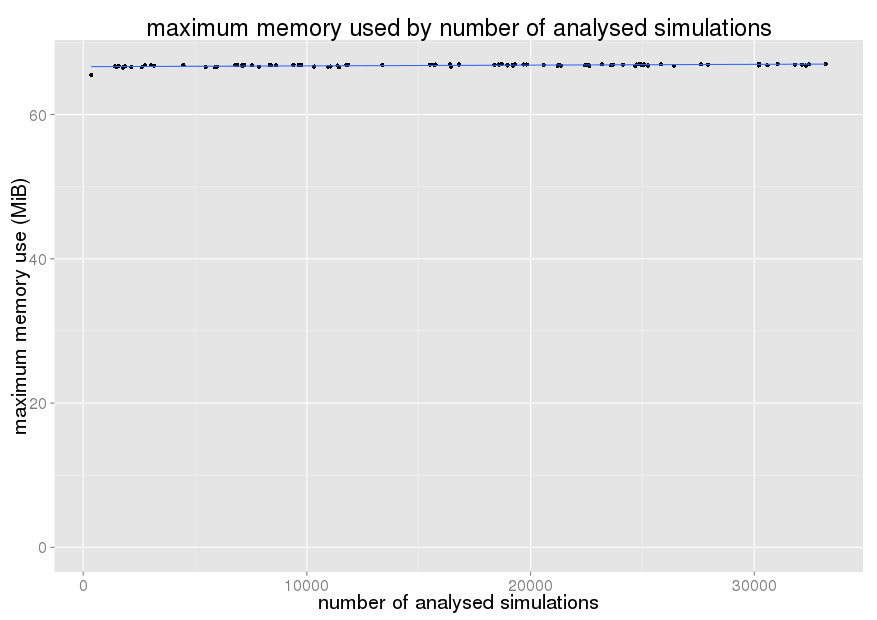
\includegraphics[width=0.585\textwidth]{../data/merge-maxMemByNSimulations.png}
\end{figure}
\end{frame}

\begin{frame}[plain, noframenumbering]{}{Benchmark \texttt{analysis} \& \texttt{ABC}}
\begin{figure}
  \hspace*{-1cm}
  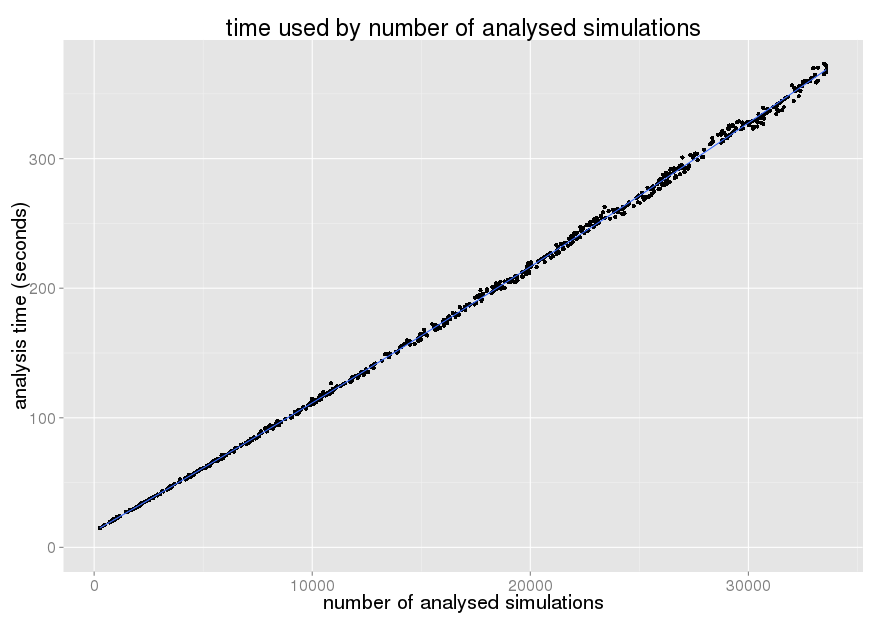
\includegraphics[width=0.585\textwidth]{../data/analysis-timeByNSimulations.png}%
  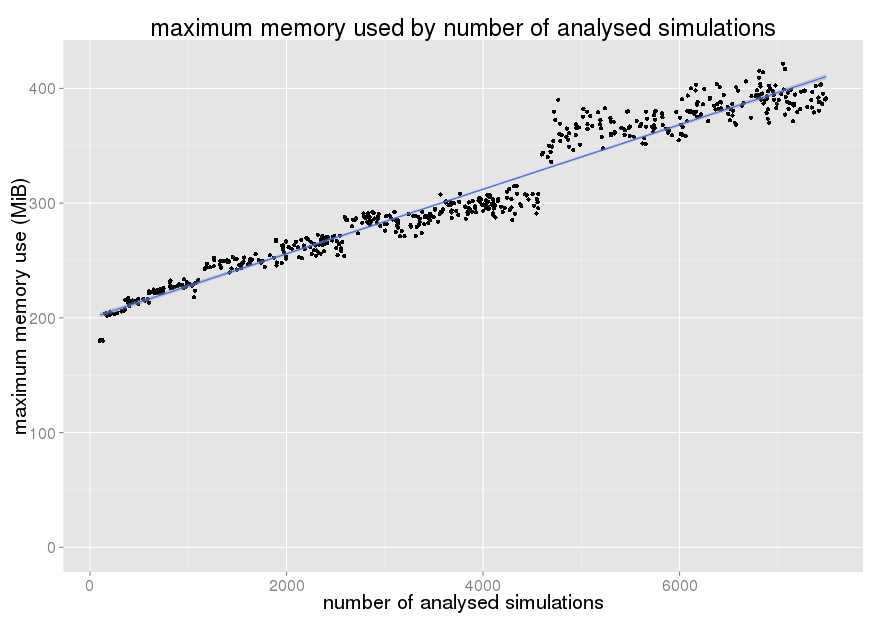
\includegraphics[width=0.585\textwidth]{../data/analysis-maxMemByNSimulations.png}
\end{figure}
\end{frame}

\end{document}
